%%%%%%%%%%%%%%%%%%%%%%%%%%%%%%%%%%%%%%%%%%%%%%%%%%%%%%%%%%%%%%%%%%%%%%%%%%%%%%%%
%2345678901234567890123456789012345678901234567890123456789012345678901234567890
%        1         2         3         4         5         6         7         8

%\documentclass[letterpaper, 10pt, conference]{ieeeconf}  % Comment this line out if you need a4paper

\documentclass[a4paper, 10pt, conference]{ieeeconf}      % Use this line for a4 paper

% \IEEEoverridecommandlockouts                              % This command is only needed if 
                                                          % you want to use the \thanks command

\overrideIEEEmargins                                      % Needed to meet printer requirements.

%In case you encounter the following error:
%Error 1010 The PDF file may be corrupt (unable to open PDF file) OR
%Error 1000 An error occurred while parsing a contents stream. Unable to analyze the PDF file.
%This is a known problem with pdfLaTeX conversion filter. The file cannot be opened with acrobat reader
%Please use one of the alternatives below to circumvent this error by uncommenting one or the other
%\pdfobjcompresslevel=0
%\pdfminorversion=4

% See the \addtolength command later in the file to balance the column lengths
% on the last page of the document

% The following packages can be found on http:\\www.ctan.org
%\usepackage{graphics} % for pdf, bitmapped graphics files
%\usepackage{epsfig} % for postscript graphics files
%\usepackage{mathptmx} % assumes new font selection scheme installed
%\usepackage{times} % assumes new font selection scheme installed
%\usepackage{amsmath} % assumes amsmath package installed
%\usepackage{amssymb}  % assumes amsmath package installed
\usepackage{amsfonts,amssymb} 
\usepackage{subfigure}
\usepackage{booktabs}
\usepackage{diagbox}
\usepackage{graphicx}
\usepackage{multirow}
\usepackage{amsmath}
\usepackage{overpic}
\usepackage{epstopdf}
\usepackage{xcolor}

\usepackage{algpseudocode}

\usepackage[linesnumbered,ruled,vlined]{algorithm2e}

\usepackage{caption}
\captionsetup{font={small}}

\usepackage{etoolbox}
\makeatletter
\patchcmd{\@makecaption}
{\scshape}
{}
{}
{}
\makeatother

\title{\LARGE \bf
3D Object Detection and Tracking on Streaming Data
}


\author{Xusen Guo$^{1}$ and Kai Huang$^{2}$% <-this % stops a space
% \thanks{*This work was not supported by any organization}% <-this % stops a space
% \thanks{$^{1}$Albert Author is with Faculty of Electrical Engineering, Mathematics and Computer Science, 
% University of Twente, 7500 AE Enschede, The Netherlands {\tt\small albert.author@papercept.net}}%
% \thanks{$^{2}$Bernard D. Researcheris with the Department of Electrical Engineering, 
% Wright State University, Dayton, OH 45435, USA {\tt\small b.d.researcher@ieee.org}}%
}

\def\eg{\emph{e.g.}}
\def\Eg{\emph{E.g.}}
\def\etal{\emph{et al. }}
\def\figurename{\emph{Figure}}
\def\tablename{\emph{Table}}

\begin{document}

\maketitle
\thispagestyle{empty}
\pagestyle{empty}


%%%%%%%%%%%%%%%%%%%%%%%%%%%%%%%%%%%%%%%%%%%%%%%%%%%%%%%%%%%%%%%%%%%%%%%%%%%%%%%%
\begin{abstract}

Recent approaches for 3D object detection have made tremendous progresses due to the development of deep learning. However, previous researches are mostly based on single frame input, information between frames is scarcely explored. In this paper, we attempt to leverage the temporal information in streaming data and explore 3D streaming based object detection as well as tracking. Toward this goal, we set up a dual-way network for 3D object detection in keyframes only, and then propagate predictions to non-key frames through a motion based interpolation algorithm guided by temporal information. Our proposed framework is shown to have great improvements on object detection compared to frame-by-frame approach, and also proven to produce competitive results on the KITTI Object Tracking Benchmark, with 76.68\% in MOTA and 81.65\% in MOTP respectively.

%Meanwhile, a \textit{Temporal module} is introduced to capture object co-occurrence and offsets across frame.

%Towards this goal, we set up a network that can associate image features and point cloud features in keyframes to generate accurate 3D detections and trajectories in an end-to-end form. Specifically, a Temporal module is introduced to capture object co-occurrence across time, and a motion based interpolation algorithm is proposed to generate streaming level predictions. Our proposed architecture is proven to produce competitive results on the KITTI Object Tracking Benchmark, with 76.68\% in MOTA and 81.65\% in MOTP respectively.
\end{abstract}

%%%%%%%%%%%%%%%%%%%%%%%%%%%%%%%%%%%%%%%%%%%%%%%%%%%%%%%%%%%%%%%%%%%%%%%%%%%%%%%%
\section{INTRODUCTION}

3D Object detection has received increasing attention over the last few years due to the rapid development of autonomous driving. Compared to 2D image, 3D data can provide accurate location of targets and characterize their shapes. Current approaches for 3D object detection are mostly carried out in three fronts: image based \cite{7780605, chen20183d}, point clouds based \cite{zhou2018voxelnet,yang2018pixor,simon2018complex}, and multi-view fusion based \cite{chen2017multi,ku2018joint}. Most of these approaches have achieved competitive results but are limited to single frame input.

During autonomous driving, data is always obtained in a streaming fashion, thus it's more natural to perform object detection with streaming data. Compared to single frame, streaming data can provide consistent temporal correlations between consecutive frames for detected features, which can reduce noisy detections over time. In addition, truncated and occluded targets can possibly be compensated by subsequent frames within streaming data. Therefore, exploring 3D object detection methods specifically for streaming data is essential and promising.

Performing 3D object detection in streaming data is however complex. First of all, acquiring consistent 3D information between frames is difficult. On the one hand, camera data provide rich appearance features but lack of depth information. On the other hand, though LiDAR can accurately detect the position of object of interest, it is very sparse and thus difficult to determine the appearance of object purely from its point cloud representation. Second, how to correlate the features between individual frames is not obvious. For example, generating 3D scene flow with temporal feature representation will need to determine the corresponding points between frames, which is not straightforward and also challenging. Last but not least, the sheer numbers of frames that streaming data provided introduce tremendous computational costs, especially for real-time applications. 

This paper proposes a \textbf{D}ual-way \textbf{O}bject \textbf{D}etection and \textbf{T}racking (\textbf{DODT}) framework, as is illustrated in \figurename \, \ref{fig:dodt}, to tackle aforementioned problems. We construct our framework based on the following observations: (1) streaming data is huge but redundant, thus we can process keyframes only and propagate predictions to non-key frames. (2) object detection can be benefit from long-term information which can be obtained through cross-correlation between adjacent frames, as demonstrated in \cite{feichtenhofer2017detect}. For first observation, we design our framework into a dual-way fashion, thus it can operate two adjacent keyframes simultaneously and convenient for prediction propagation. Moreover, a specific network named \textit{Shared RPN} is proposed to generate 3D proposals to be shared by two detection branches. For second observation, a \textit{Temporal module} is introduced to capture temporal information through cross-correlation in BEV space, and then predicts object co-occurrence and offsets between two keyframes. Notably, different from \cite{feichtenhofer2017detect, dosovitskiy2015flownet},  our correlation operation is performed on proposal level, which leads to a much less computational cost. 

To generate predictions of every frame, a motion based interpolation algorithm is developed to propagate keyframe predictions to non-key frames guided by \textit{Temporal module} outputs. Meanwhile, multi-object tracking can also be accomplished through \textit{tracking by detection} \cite{lenz2015followme}. In summary, our contributions are threefold:
\begin{itemize}
	\item We propose a dual-way framework named DODT,  which performs 3D object detection and tracking precisely on streaming data by only processing keyframes.
	\item A \textit{Temporal module} is proposed to encode temporal information across frame in proposal level, which is much efficient than previous approaches.
	\item A motion based interpolation algorithm is developed for prediction propagation, which leads to considerable performance improvements in object detection and tracking.  
\end{itemize}

%\textit{(i)} We set up a dual-way framework for 3D streaming based object detection and tracking, which only processes keyframes and propagate  \textit{(ii)} We introduce  \textit{Temporal module} for temporal object cross-correlation representation, which is much efficient than previous approaches. \textit{(iii)} We develop a motion based interpolation algorithm for streaming level detection and tracking, which leads to considerable improvements on both tasks.  


%of our approach is that object detection can be benefit from long-term information which can be obtained through convolutional cross-correlation between adjacent frames, as demonstrated in \cite{feichtenhofer2017detect}. 

% Our DODT framework (as illustrated in \figurename \, \ref{fig:dodt}) consists of a \textit{Shared RPN module}, two detection branches, a \textit{Temporal module} and a motion based interpolation algorithm. First, the \textit{Shared RPN module} generates 3D proposals shared by two detection branches fed with features of consecutive frames. With 3D proposals, the detection branch then aggregates features from point cloud view and image view, and output predictions of key frame precisely. At the same time, \textit{Temporal module} utilizes correlation operation to encode temporal features in BEV space and predicts object co-occurrence and offsets between two key frames. Finally, the interpolation algorithm is applied to propagate key frame predictions to non-key frames guided the output of \textit{Temporal module}. 

%Our DODT framework performs streaming based object detection by only process key frames, while results of non-key frames are generated by interpolation guided by temporal information. Meanwhile, multi-object tracking can also be accomplished through \textit{tracking by detection} \cite{lenz2015followme}. In summary, our contributions are threefold: \textit{(i)} We set up a dual-way network for 3D streaming based object detection and tracking in autonomous driving scenarios. \textit{(ii)} We introduce a \textit{Temporal module} for temporal object cross-correlation representation, which is much efficient than previous approaches. \textit{(iii)} We develop a motion based interpolation algorithm for streaming level detection and tracking, which leads to considerable improvements on both tasks.

%The structure of \textbf{DODT} is illustrated in \figurename \, \ref{fig:dodt}, consisting of a \textit{shared RPN module}, two detection branches and a \textit{Temporal module}. The \textit{shared RPN module} is fed with two keyframes and the frames between them, and output 3D proposals shared by two detection branches. The detection branch aggregates point cloud features with image features, and predict class and bounding box of the object of interest precisely. While \textit{Temporal module} utilizes correlation operation to encode temporal features in BEV space and predicts object co-occurrence and displacement between two keyframes. Notably, different from \cite{feichtenhofer2017detect, dosovitskiy2015flownet}, our correlation operation is performed on proposal level supported by \textit{shared RPN module}, which leads to a much less computational cost. Note that object detection is only performed on keyframes, in order to obtain results of all frames, we develop a motion based interpolation algorithm to propagate keyframes predictions to non-key frames. Meanwhile, multi-object tracking can also be accomplished through \textit{tracking by detection} \cite{lenz2015followme} paradigm. Aided with \textit{Temporal module}, our interpolation algorithm also shows a good solution for some typical tracking problems such as object drift, loss of targets in one frame, etc., which other researches suffer a lot.

%In summary, our contributions are threefold: \textit{(i)} We set up a dual-way network for 3D streaming based object detection and tracking in autonomous driving scenarios. \textit{(ii)} We introduce a \textit{Temporal module} for temporal object cross-correlation representation, which is much efficient than previous approaches. \textit{(iii)} We develop a motion based interpolation algorithm for streaming level detection and tracking, which leads to considerable improvements on both tasks. 

%We perform our approach to KITTI Object Tracking Benchmark and obtain competitive results, with 72.21\% in MOTA and 82.29\% in MOTP respectively.

%The network has a RPN module to generate 3D proposals and two detection branches to perform 3D object detection on two adjacent keyframes respectively. To compensate for the sparsity of point cloud data, the network aggregates image features and thus can utilize the strengths of both. Considering the redundancy of features between frames, the 3D proposals are shared by two detection branches. In order to avoid estimating 3D scene flow directly when computing object cross-correlation features, a Temporal module is aided to our network for temporal feature encoding. The Temporal module uses correlation operation to extract temporal features and predict object displacements over keyframes, but different from traditional ways which performed on whole feature maps, it does correlation on object proposal-level with the help of sharing mechanism in proposals. 

%For a fast inference speed, we only performs object detection on keyframes and propagate predicted bounding boxes to neighboring frames for a streaming-based detection. By linking detections over time, multi-object tracking can be finished through \textit{tracking by detection} \cite{lenz2015followme}. Note that tracking using two frames often suffers from many problems, such as drift, loss of targets in one frame, etc. We develop a interpolation algorithm driven by motion model to address these problems. The ablation study shows the effectiveness of our interpolation algorithm.
%%%%%%%%%%%%%%%%%%%%%%%%%%%%%%%%%%%%%%%%%%%%%%%%%%%%%%%%%%%%%%%%%%%%%%%%%%%%%%%%
\begin{figure*}
	\vspace{-0.6cm}
	\rule{0pt}{1ex}
	%\setlength{\abovecaptionskip}{-0.1cm}
	\begin{center}
		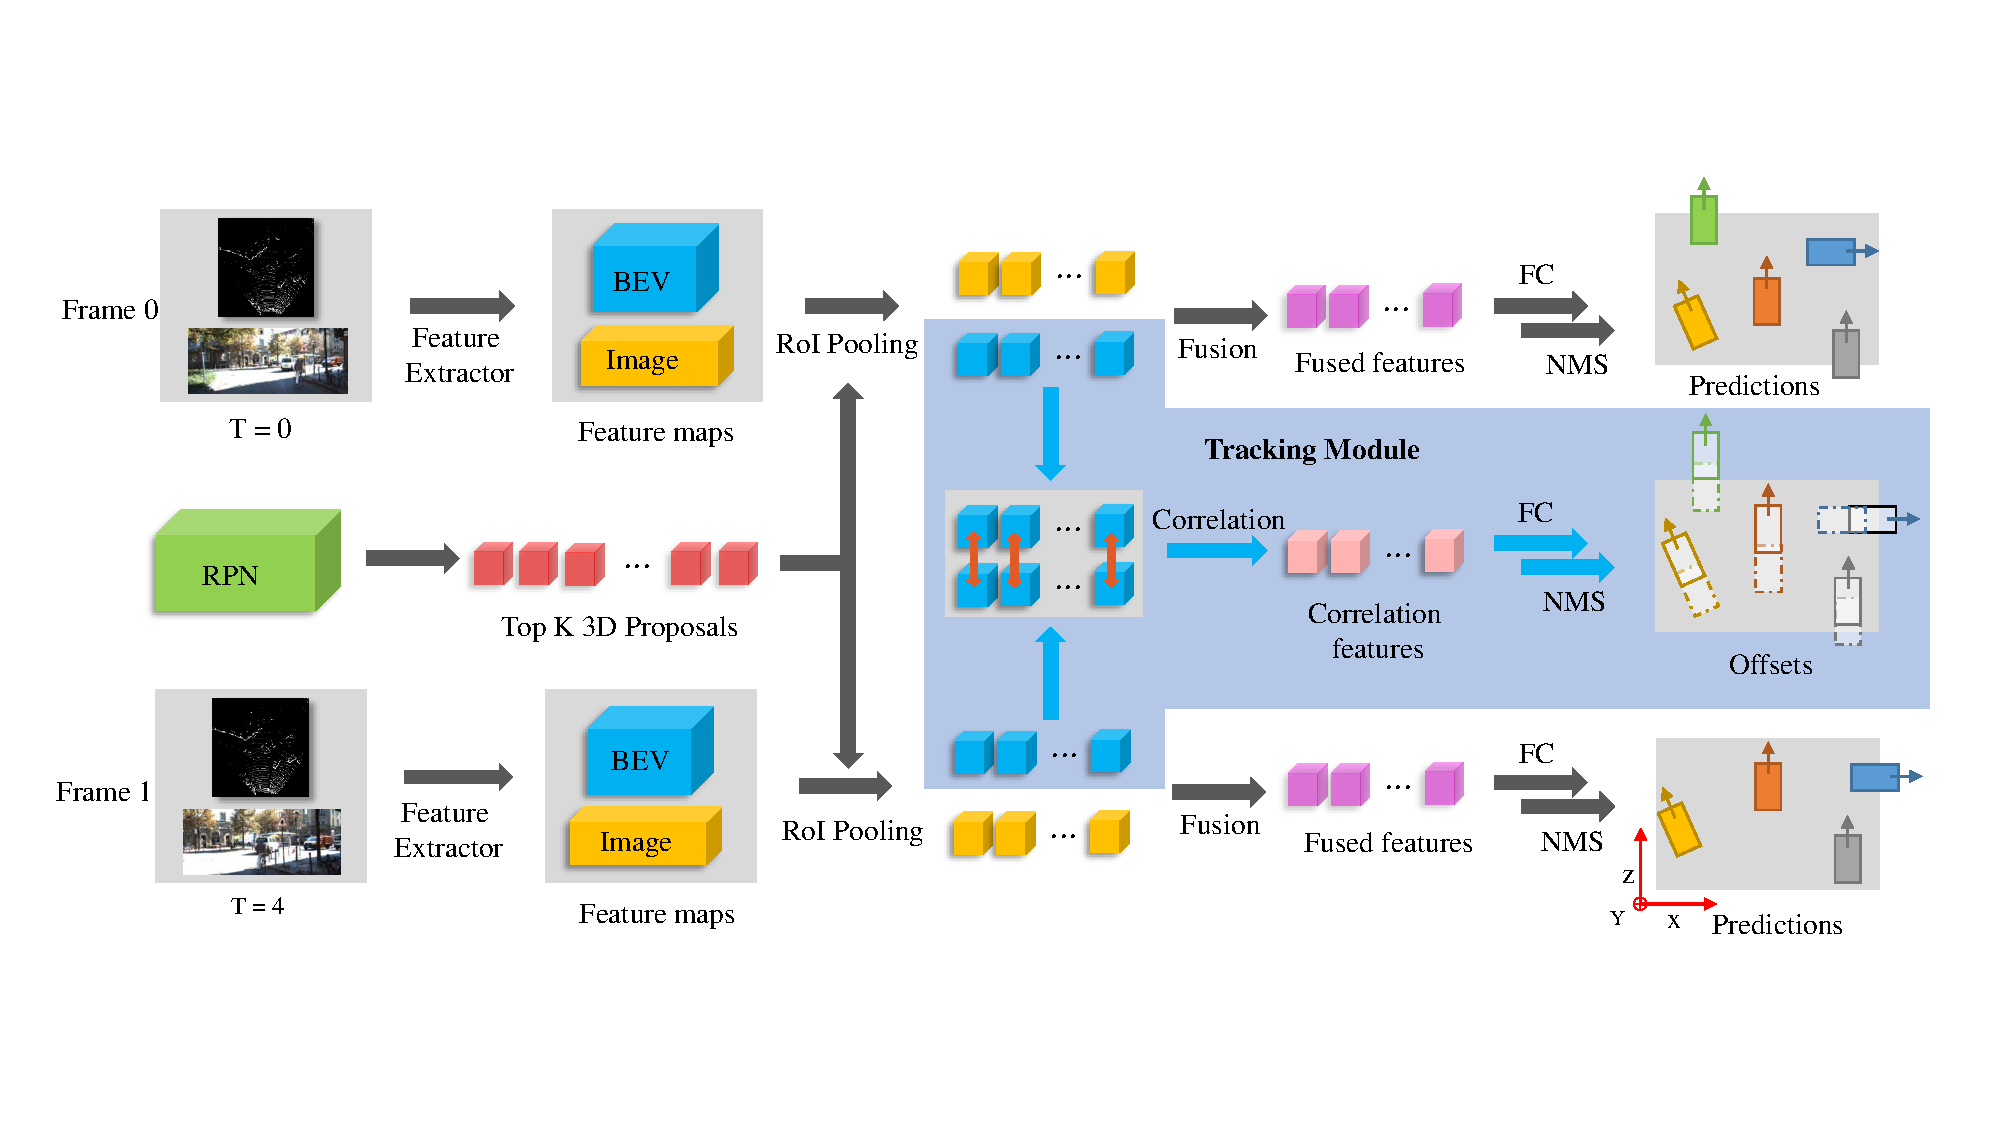
\includegraphics[trim={0.5cm, 3cm, 0.5cm, 3cm}, clip, width=\textwidth]{images/structure.pdf}
	\end{center}
	\caption{DODT architecture. Blue area is \textit{Temporal module}, it does not use image features since information in BEV is sufficient for tracking.}
	\label{fig:dodt}
	\vspace{-0.5cm}
\end{figure*}

\section{RELATED WORK}

\textbf{3D object detection.} Currently, most approaches in 3D object detection are usually done in three fronts: image based, point cloud based, and multi-view fusion based. Image based approaches such as Mono3D \cite{7780605} and 3DOP \cite{chen20183d} use camera data only. Since image lacks depth information, hand-crafted geometric features are required in these approaches. As for the point cloud based methods, there are usually two ways: voxelization based and projection based, according to how point clouds features are represented. Voxelization based methods such as 3D FCN \cite{li20173d}, Vote3Deep \cite{engelcke2017vote3deep}, VoxelNet \cite{zhou2018voxelnet}, utilize a voxel grid to encode features. These approaches suffer from the sparsity of point clouds and enormous computation costs in 3D convolution. While projection based methods such as PIXOR \cite{yang2018pixor}, Complex-YOLO \cite{simon2018complex}, Complexer-YOLO \cite{Simon_2019_CVPR_Workshops} attempt to project point clouds to a perspective view (e.g. bird eye view) and apply image-based feature extraction techniques. However, due to the sparsity of point clouds, features after projection are usually insufficient for accurate object detection, especially for small targets. Multi-view fusion based approaches such as F-PointNet \cite{qi2018frustum}, MV3D \cite{chen2017multi}, AVOD \cite{ku2018joint}, try to fuse point cloud features with image features for accurate object detection. These methods distinguish from each other mainly on how data is fused. Our detection branches are constructed based on AVOD, but proposal features are enhanced with temporal information.

%first extracts the 3D bounding frustum of an object by extruding 2D bounding boxes from image detectors, then consecutively performs 3D object instance segmentation and amodal extent regression to estimate the amodal 3D bounding box. This method works well for indoor scenes and brightly lit outdoor scenes, but are expected to perform poorly in more extreme outdoor scenarios. MV3D \cite{chen2017multi} extends the image based RPN of Faster R-CNN\cite{ren2015faster} to 3D and proposes a 3D RPN, then applies feature fusion of images and point clouds to produces accurate 3D detections. However, due to the insufficient information in feature extraction caused by downsampling, it does not work well for small targets. AVOD \cite{ku2018joint} is similar to MV3D in 3D RPN and feature fusion, but with  full resolution feature maps produced by a pyramid architecture, which leads to a great improvement in localization accuracy for small targets. Our detection submodule is somehow similar to AVOD, but enhances proposal's feature with temporal information additionally.

\textbf{Video object detection.} Nearly all existing methods in video object detection incorporate temporal information on either feature level or final box level. FGFA \cite{zhu2017flow} leverages temporal coherence on feature level, it warps the nearby frames feature maps to a reference frame for feature enhancement according to flow emotion. On the other hand, T-CNN \cite{kang2018t, kang2016object} leverages precomputed optical flows to propagate predicted bounding boxes to neighboring frames; Seq-NMS \cite{han2016seq} improves NMS algorithm for video by constructing sequences along nearby high-confidence bounding boxes from consecutive frames. They are all utilize temporal information in final box level. There are also a few approaches attempt to learn temporal features between consecutive frames without optical flow. D\&T \cite{feichtenhofer2017detect} proposes a two branches detection network for object detection and tracking simultaneously in video. The network learns temporal information representation through computing convolutional cross-correlation between frames. Our DODT approach is mainly inspired by D\&T, however, we develop this idea to 3D space and restrain correlation operation in proposal level, which reduce computational costs significantly. Moreover, tracking using two adjacent frames often suffers from drift, loss of targets in one frame, etc., our approach can handle these issues well by performing motion based interpolation algorithm.

%uses a detection and tracking based loss for simultaneous detection and tracking in video. In order to learn temporal information representation, the network is fed with multiple frames, and a correlation module is embedded for computing convolutional cross-correlation between frames. Our DODT approach is mainly inspired by D\&T, however, we develop this idea to 3D space. Moreover, we constrain correlation operation in proposal-level, which reduce computational costs significantly. 

%it first applies feature extraction network on individual frames to produce per-frame feature maps, and then enhances features at a reference frame by warping the nearby frames feature maps according to flow emotion. 
%On the other hand, final box level approaches usually utilize temporal information in bounding box post processing. T-CNN \cite{kang2018t, kang2016object} leverages precomputed optical flows to propagate predicted bounding boxes to neighboring frames, and then generates tubelets by applying tracking algorithms from high-confidence bounding boxes. Seq-NMS \cite{han2016seq} improves NMS algorithm for video by constructing sequences along nearby high-confidence bounding boxes from consecutive frames. While boxes of the sequence are then re-scored to the average confidence and other boxes close to this sequence are suppressed. 

%Other approaches such as D\&T \cite{feichtenhofer2017detect} attempt to learn temporal features between consecutive frames to avoid using optical flow. D\&T \cite{feichtenhofer2017detect} uses a detection and tracking based loss for simultaneous detection and tracking in video. In order to learn temporal information representation, the network is fed with multiple frames, and a correlation module is embedded for computing convolutional cross-correlation between frames. Our DODT approach is mainly inspired by D\&T, however, we develop this idea to 3D space. Moreover, we constrain correlation operation in proposal-level, which reduce computational costs significantly. 

\textbf{3D multi-object tracking.} Existing 3D multi-object tracking approaches are mostly implemented based on tracking by detection. For example, FaF \cite{luo2018fast} jointly reasons about 3D detection, tracking and motion forecasting taking a 4D tensor created from multiple consecutive temporal frames. It can aggregate the detection information for the past $n$ timestamps to produce accurate tracklets. 3D-CNN/PMBM \cite{scheidegger2018mono} trained a DNN to detect and estimate the distance to objects from a single image, and then fed the detections to a Poisson multi-Bernoulli mixture tracking filter for 3D tracking. DSM \cite{frossard2018end} first predicts 3D bounding boxes in continuous frames and then associates detections using a \textit{Matching net} and a \textit{Scoring net}, which is similar to our approach. However, their 3D detector is directly single frame based approach MV3D \cite{chen2017multi}, temporal features between frames are mostly ignored. Moreover, their bounding boxes association is done by solving a linear program and is an offline version, while our tracking algorithm is an near online approach.

%%%%%%%%%%%%%%%%%%%%%%%%%%%%%%%%%%%%%%%%%%%%%%%%%%%%%%%%%%%%%%%%%%%%%%%%%%%%%%%%

\section{METHODOLOGY}

In this section, we first give an overview of our DODT approach (Sec. A) that performs 3D object detection and tracking given two adjacent keyframes as inputs. We then introduce the \textit{shared RPN} (Sec. B) that generates 3D proposals shared by two detection branches. Sec. C shows how \textit{Temporal module} encodes cross-correlation features and predicts the co-occurrence and displacement of corresponding targets in two adjacent keyframes. Sec. D shows how we implement motion based interpolation algorithm and accomplish 3D streaming based object detection and multi-object tracking simultaneously.

\subsection{DODT Model Structure} 

We aim at performing 3D object detection and tracking on streaming data. To this end, we design DODT into a dual-way network. \figurename \, \ref{fig:dodt} illustrates the whole pipeline. With the help of the dual-way structure, the network can fed with two adjacent keyframes data simultaneously. The keyframes data consists of an image and point cloud BEV maps (following the procedure described in MV3D \cite{chen2017multi}). Keyframe data is first fed to a feature extractor to get corresponding feature maps. The feature extractor is designed following the procedure described in AVOD \cite{ku2018joint}, which constructed in an encoder-decoder fashion resulting in a full resolution feature map. To extract feature crops from image and BEV feature maps, we also follow the idea proposed in AVOD. Given a 3D anchor generated by RPN, two view specific ROIs are obtained by projecting the anchor onto the image and BEV feature maps, the corresponding feature crops are extracted and then RoI pooling is performed from two views. After that, a \textit{early fusion} scheme in MV3D \cite{chen2017multi} is used to combine multi-view features in proposal level. Finally, after applying fully connected layers for classification and box regression, and 2D non-maximum suppression (NMS) for proposals filtering, the final predictions are produced. Meanwhile, fed with BEV feature crops of two branches, \textit{Temporal module} performs correlation operation on feature crop pairs to produce cross-correlation features. The cross-correlation features are then used to predict object co-occurrence and displacement between two keyframes for streaming-level detection and tracking.

The whole network is designed in an end-to-end form. The multi-task objective consists of a cross-entropy loss $L_{cls}$ for classification, a smooth \textit{L1} loss $L_{reg}$ for box regression, and a smooth \textit{L1} loss $L_{corr}$ for displacement regression between corresponding objects across two keyframes. $L_{reg}$ and $L_{corr}$ are normalized by the number of proposals while $L_{cls}$ is normalized by the number of positive proposals.

\subsection{Shared RPN}

\begin{figure}
	\vspace{-0.6cm}
	\rule{0pt}{1ex}
	%\setlength{\abovecaptionskip}{-0.1cm}
	\begin{center}
		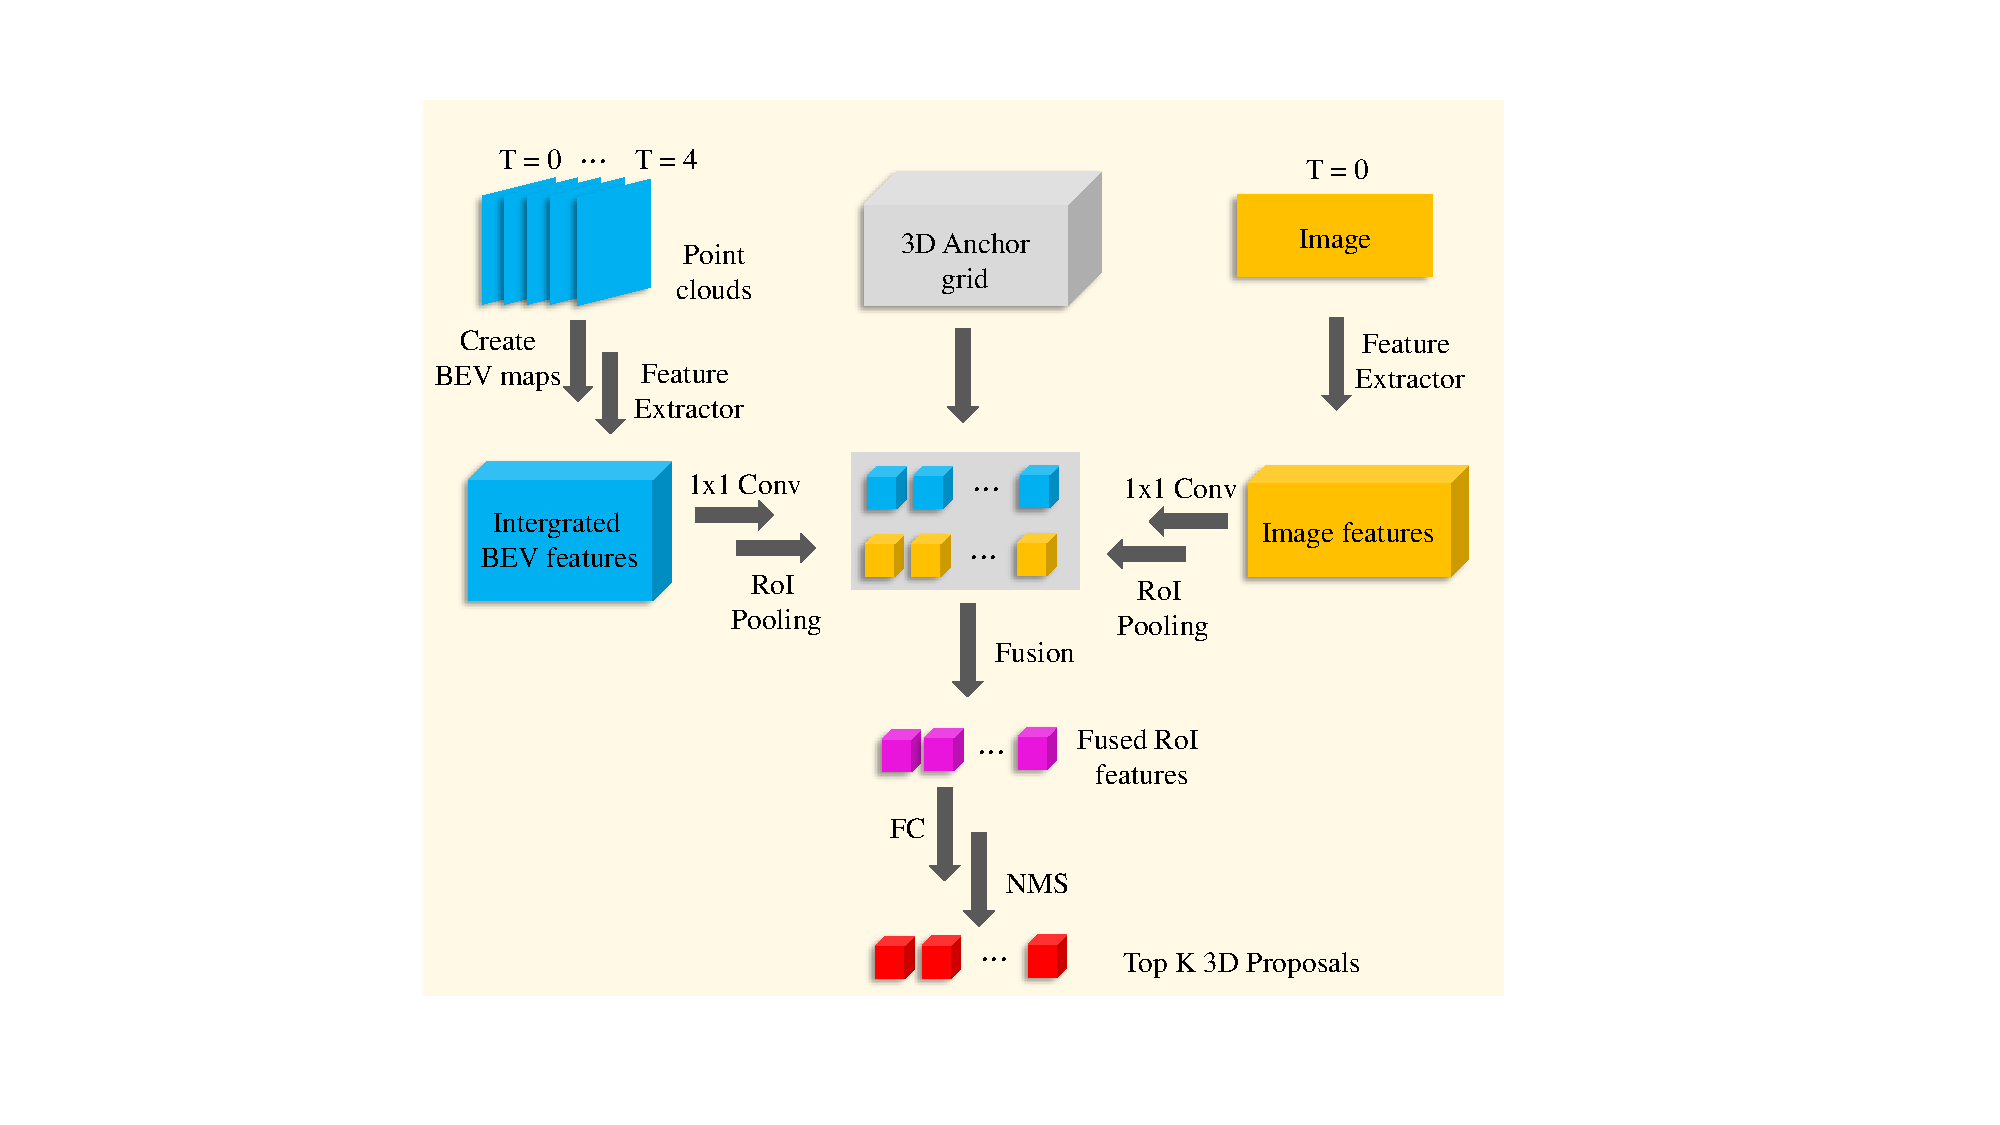
\includegraphics[trim={7cm, 2cm, 7.8cm, 2cm}, clip,width=0.45\textwidth]{images/rpn.pdf}
	\end{center}
	\caption{Shared RPN module.}
	\label{fig:rpn}
	\vspace{-0.5cm}
\end{figure}

\begin{figure}
	\vspace{-0.6cm}
	\rule{0pt}{1ex}
	\begin{center}
		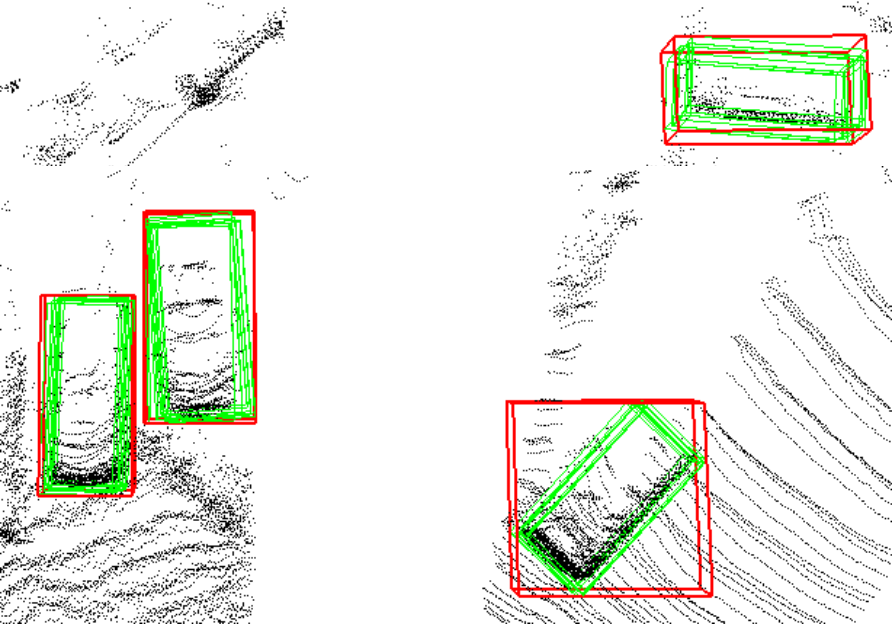
\includegraphics[width=0.45\textwidth]{images/integrated_boxes.png}
	\end{center}
	\caption{Five consecutive point clouds in the same coordinate system. Green boxes are default labels of five frames, while red boxes are the axis-aligned new labels for RPN training.}
	\label{fig:integrated_boxes}
	\vspace{-0.6cm}
\end{figure}

We transform RPN network in AVOD \cite{ku2018joint} to our \textit{shared RPN network} (as shown in \figurename \, \ref{fig:rpn}), which can generate 3D proposals shared by both detection branches. To ensure proposals generated by our RPN are suitable for both keyframes, we create integrated BEV feature maps based on two keyfames and the frames between them. Note that point cloud shows object accurate 3D localization, we can simply transform these frames to a same coordinate system and then fuse them. Since point cloud is extremely sparse and is encoded by projection, this process does not increase any computational cost but enhance the point cloud BEV feature maps greatly. Assume there are five frames in point cloud input, due to object movement, the location of the same object in five frames are shift. For training convenient, we replace original proposal labels with new axis-aligned labels that can cover all five original labels of an object in five frames. \figurename \, \ref{fig:integrated_boxes} illustrates these two kind of labels. Though this process enlarges proposal labels, it can ensure that new labels are suitable for proposal prediction in both detection branches. Moreover, to obtain accurate proposals, We fuse BEV feature maps with image data to enhance object appearance features. Since one image contains enough features in a short temporal slice, our module only aggregates the features in first image of a slice. Subsequent processing and operations are similar with RPN module described in AVOD, we refer the reader to \cite{ku2018joint} for more information.

\subsection{Temporal Module}
The \textit{Temporal Module} is demonstrated in \figurename \, \ref{fig:dodt}. Given two sets of point cloud BEV features crops $F_t, F_{t+\tau}$, a set of cross frame feature pairs can be constructed as $\{(F_t^i, F_{t+\tau}^i)\mid i \in \{0,1,...,N\}\}$, where $F_t^i, F_{t+\tau}^i$ are features extracted by $i$-th proposal from frame $t$ and frame $t+\tau$ respectively, $\tau$ is temporal stride and $N$ is the number of 3D proposals. Note that proposals generated by RPN are shared by two detection branches, thus the set can be obtained conveniently. After the correspondence of feature crops is constructed, correlation operation can be performed on feature pair $(F_t^i, F_{t+\tau}^i)$ to compute cross-correlation features over frames. Once the cross-correlation features are obtained, they are fed to a classification head for object co-occurrence prediction and a regression head for box offsets prediction respectively. Object co-occurrence determines whether an object exists on both keyframes, it provides an extra guarantee for the successful implementation of the interpolation algorithm. When an object is loss in one of the two keyframes, object co-occurrence shows the probability of a mis-detection, or a track start or end. More details are available in Sec. D.

For a target we have ground truth $d^t = (p_{co}, d^t_x, d^t_z, d^t_{ry})$ in frame $t$ for \textit{Temporal Module}, and similarly $d^{t+\tau}$ for frame $t+\tau$, denoting object co-occurrence probability and its horizontal and vertical center coordinates as well as orientation in BEV map. $p_{co}$ is 1 if the target exists on both keyframes, 0 otherwise. The box offsets label $\Delta^{t, t+\tau} = (\delta^{t,t+\tau}_{x}, \delta^{t,t+\tau}_{z}, \delta^{t,t+\tau}_{ry})$ is then
%\vspace{-0.3cm}
\begin{equation}
%\scriptsize
%(\delta_{x}^{t, t+\tau}, \delta_{z}^{t, t+\tau}, \delta_{ry}^{t, t+\tau}) = 
\Delta^{t, t+\tau} =
\begin{cases}
(\frac{d_{x}^{t+\tau} - d_{x}^{t}}{d^t_{w}}, \frac{d_{z}^{t+\tau} - d_{z}^{t} }{d^t_{l}}, \frac{d_{ry}^{t+\tau} - d_{ry}^{t}}{d^t_{ry}}) & d \in F_t \cap F_{t+\tau} \\
(0.0,0.0, 0.0) &  otherwise
\end{cases}
\end{equation}
where $d^t_{w}, d^t_{l}$ are width and height of the object.
%\begin{equation}
%\small
%(\delta_{l}^{t, t+\tau}, \delta_{w}^{t, t+\tau}) = 
%\begin{cases}
%(0.0,0.0) & d \in F_t \cap F_{t+\tau} \\
%(1.0, 1.0) & d \notin F_t \cap d \in F_{t+\tau} \\
%(-1.0, -1.0) & d \in F_t \cap d \notin F_{t+\tau}
%\end{cases}
%\end{equation}
%If the target exists in both keyframes, the shape offsets $(\delta^{t,t+\tau}_{l}, \delta^{t,t+\tau}_{l})$ are zero since 3D shape of vehicle dose not change over time. \textit{Temporal Module} only need to predict location offsets $(\delta^{t,t+\tau}_{x}, \delta^{t,t+\tau}_{z}, \delta^{t,t+\tau}_{ry})$. If the target exists only in one keyframe, we set location offsets to zero but shape offsets to 1 for target appearance and -1 for disappearance. The encoding of object existence is the key technology to determine a birth or death of a trajectory, more details are available in Sec. D.


%Considering 3D shape of vehicle dose not change over time, and displacement information can be well represented by BEV feature maps, \textit{Temporal Module} only predicts X-axis, Z-axis offsets $(\Delta^{t,t+\tau}_{x}, \Delta^{t,t+\tau}_{z})$ of object center and steering angle  $\Delta^{t,t+\tau}_{ry}$. This is also why we use BEV feature crops only in \textit{Temporal Module}. In order to address object mismatch caused by tracklet birth or death, the module output a pair of offsets $(\Delta^{t, t+\tau},\Delta^{ t+\tau, t})$ corresponding to two keyframes. For an object exists only in one keyframe, its unique displacement can be used to determine whether a true start or end of a trajectory occurs, or just the instability of the model should be responsible for. More details are available in Sec. D.

%\begin{figure}
%	\vspace{-0.6cm}
%	\rule{0pt}{1ex}
%	\begin{center}
%		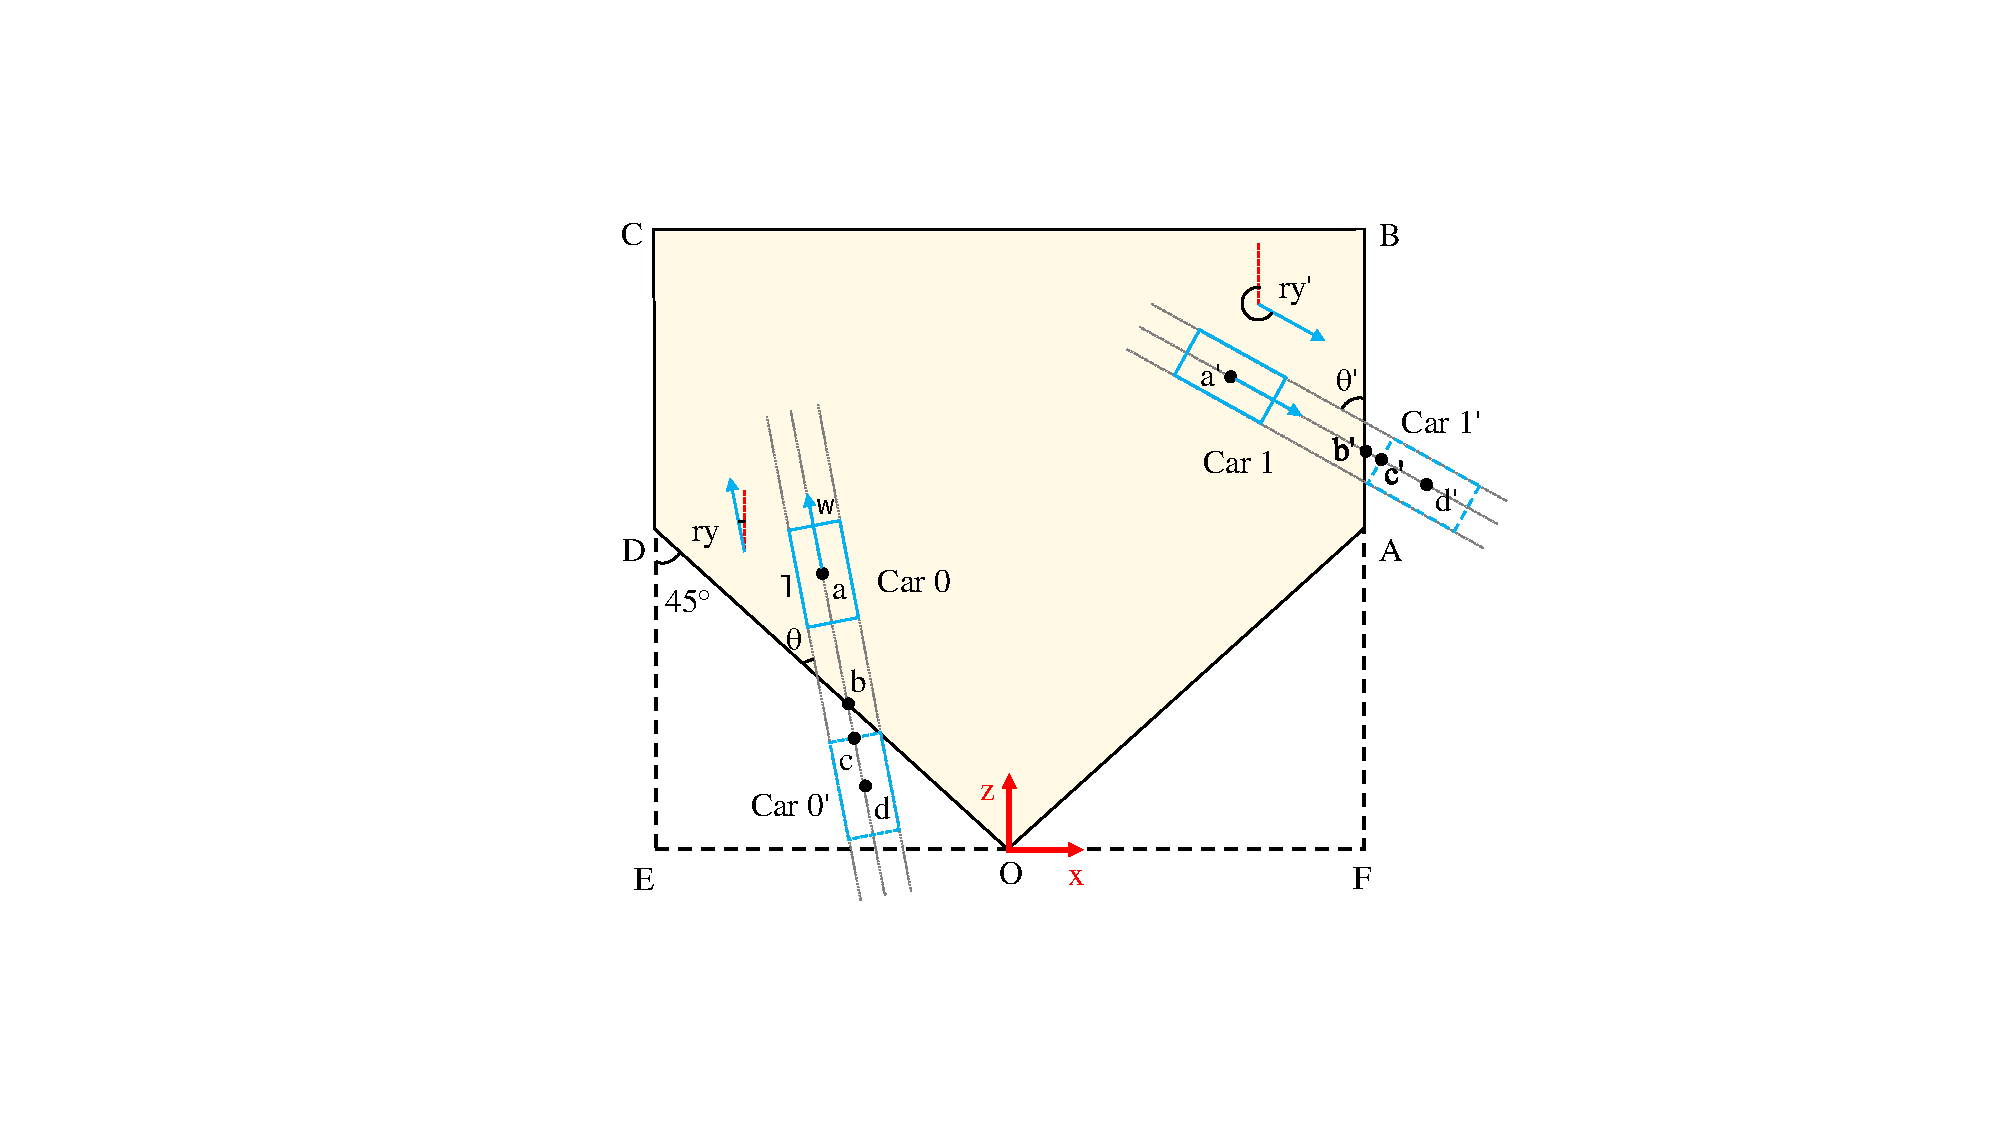
\includegraphics[trim={10cm, 4cm, 8cm, 3.5cm}, clip, width=0.5\textwidth]{images/motion.pdf}
%	\end{center}
%	\caption{Motion model of objects that in the start or end of a trajectory.}
%	\label{fig:motion}
%	\vspace{-0.6cm}
%\end{figure}

\subsection{3D Streaming Object Detection and Tracking}
Since streaming data possesses a lot of redundant information and objects typically move smoothly in time, we can perform detection network on keyframes and propagate results to the rest of the frames by applying  Algo. \ref{alg:interpolation}. Fed with two detections lists $D^t, D^{t+\tau}$ and a offsets list $\Delta^{t, t+\tau}$ of keyframes, the algorithm first utilizes linear interpolation to calculate detections in intermediate frames if an object exists on both keyframes. The association of detections is determined by \textit{getMatched} function, which performs a 3D IoU based algorithm with a threshold 0.2 to select the best matched detection in second keyframe given a rectified detection ($d_i^t + \delta_i^t$) in first keyframe. If match failed, the function output none. As for a detection that exists only in one keyframe, if its co-occurrence probability $p_{co}^i$ is less than $p_{co}^{max}$ (0.5 in our experiment), we regard it as a mis-detection in another keyframe, then we apply linear interpolation to propagate the detection to intermediate frames as well as another keyframe using offsets prediction $\delta^{t, t+ \tau}_i$. Otherwise we think a trajectory birth or death happens, then a motion model is leveraged to propagate the detections.

The motion model holds the hypothesis that the target velocity is constant within a short time period, independent of camera ego-motion. Thus we can calculate target state in next frame using historical state and increment. In detail, we maintain a global velocity $(v_x, v_z, v_{ry})$ in BEV space, it will be updated to $(\frac{\delta_{x}^{t, t+\tau}}{\tau}, \frac{\delta_{z}^{t, t+\tau}}{\tau}, \frac{\delta_{ry}^{t, t+\tau}}{\tau})$, once a new detection is matched with the trajectory. As for the start or end of a track, since there is no way for us to locate its head or tail with only keyframes predictions, we simply extend the track by $F_{ext}$ (3 in our experiment) frames according to the trend of movement. If the track outsides the range of BEV feature maps, then the extension will be terminated early. 

In addition, we observe that a track sometimes suffers from opposite orientation in nearby keyframes, which will lead to inferior performance. To address this issue, we operate a simple orientation correction algorithm during box interpolation and track extension. Consider a track $T^i_{match}$ and its next matched detection $D^i_{match}$, if the difference of orientation in $T^i_{match}$ and $D^i_{match}$ is grater than $\frac{\pi}{2}$, we add a $\pi$ to the orientation in $D^i_{match}$ so that its orientation can be roughly consistent with the track. 

Multi-object tracking can be accomplished with streaming level object detection simultaneously. Note that after performing interpolation algorithm on keyframe pairs, data association between keyframe pairs is also obtained. We only need to associate keyframe detections to link tracklets in time and build long-term object tubes. Since our method associates next temporal slice to the track at one time, this shows an near online tracking approach.

%The motion model is illustrated in \figurename \, \ref{fig:motion}. Rectangle BCEF is the range of selected point clouds with size of $[-40,40] \times [0, 70]$ meters along $X, Z$ axis respectively. While OABCD is the range contains points within the field of view of the camera. Taking $Car$ 0 as a example, it's a trajectory birth and is not detected in first keyframe, but is detected in second keyframe. We hold the hypothesis that $Car$ 0 is just outside OABCD and located in $d$ in first keyframe and its steering angle $ry$ is not change, thus the offset can be obtained by Equation (\ref{offsets}). Then the detections in intermediate frames can be calculated. Trajectory death case shows in $Car$ 1 can be handled in the similar way. 

\begin{algorithm}
	\small
	\caption{Motion based Interpolation Algorithm}
	\label{alg:interpolation}
	\textbf{Input: }$D^t= [d^t_0, d^t_1, ..., d^t_{N_t}], D^{t+\tau}= [d^{t+\tau}_0, d^{t+\tau}_1, ..., d^{t+\tau}_{N_{t+\tau}}],$
	$\Delta^{t, t+\tau}=[\delta^{t, t+\tau}_0, \delta^{t, t+\tau}_1, ..., \delta^{t, t+\tau}_{N}], N = max\{N_t, N_{t+\tau}\}$\\
	\textbf{Output: } $D = [D^t, D^{t+1}, ..., D^{t+\tau}]$\\
	\textbf{Initialize:} $D_{temp} = D^{t+\tau}, D, p_{co}^{max}$ \\
	\For{$d^t_i\in D^t$}{
		$d' = getMatched(d^t_i+\delta^t_i, D_{temp})$\\
		\If{$d'$}{
			$d^{t+1}_i,..., d^{t+\tau-1}_i = Interpolate(d^t_i, d')$\\
			remove $d'$ from $D_{temp}$
		}
		\ElseIf{$p_{co}^i > p_{co}^{max}$}{
			$d^{t+1}_i,..., d^{t+\tau}_i = Interpolate(d^t_i, \delta^t_i)$
		}
		\Else{predict $(d^{t+1}_i,..., d^{t+\tau-1}_i)$ by motion model}
	}
	\If{$D_{temp}$ is not empty}{
		\For{$d^{t+\tau}_j \in D_{temp}$}{
			\If{$p_{co}^j > p_{co}^{max}$}{
				$d^{t}_j,..., d^{t+\tau-1}_j = Interpolate(d^{t+\tau}_j, \delta^{t+\tau}_j)$
			}
			\Else{
				predict $(d^{t+1}_j,..., d^{t+\tau-1}_j)$ by motion model
			}
		}
	}
\end{algorithm}
\setlength{\textfloatsep}{1pt}% change space between algorithm


%\vspace{-0.2cm}
%\begin{equation}
%\begin{split}
%\mid ad \mid   &= \mid ab \mid + \mid bc \mid + \mid cd \mid  \\
% &= \mid ab \mid + \frac{w}{2tan(\frac{\pi}{4} - ry)} + \frac{l}{2}
%\end{split}
%\end{equation}
%\begin{equation}
%\{\Delta_x, \Delta_z\} = \{\mid ad \mid sin(ry), \mid ad \mid cos(ry)\}
%\label{offsets}
%\end{equation}

%For multi-object tracking, we attempt to assign each detection in each frame to a unique trajectory utilizing an extended IOU tracker algorithm\cite{bochinski2018extending}. Unlike multi-object tracking in image which suffers from boxes overlap, detection in 3D has its unique position, any overlap of two detections in BEV means high probability of the same target. Thus a IOU based data association algorithm can also work well in our approach.

%%%%%%%%%%%%%%%%%%%%%%%%%%%%%%%%%%%%%%%%%%%%%%%%%%%%%%%%%%%%%%%%%%%%%%%%%%%%%%%%
\section{EXPERIMENTS}

\begin{table*}\centering
	\small
	\resizebox{\textwidth}{!}{
		\begin{tabular}{ccccccccc}
			&\multicolumn{1}{c|}{}   & \multicolumn{3}{c|}{IoU = 0.5}  		         & \multicolumn{3}{c|}{IoU = 0.7}          &  \\ \midrule
			\multicolumn{1}{c|}{Methods} & \multicolumn{1}{c|}{Modules}    & Easy     & Moderate   & \multicolumn{1}{c|}{Hard}     & Easy  & Moderate & \multicolumn{1}{c|}{Hard}    & FPS \\\midrule
			\multicolumn{1}{c|}{AVOD\cite{ku2018joint}}     &\multicolumn{1}{c|}{-}     & 90.13 / 90.91  & 80.00 / 81.79 & \multicolumn{1}{c|}{71.61 / 81.79}  & 76.00 / 90.90 & 57.23 / 81.73 & \multicolumn{1}{c|}{56.13 / 72.69}   & 10.0\\
			\multicolumn{1}{c|}{DODT($\tau$ = 1)}     &\multicolumn{1}{c|}{-}     & 88.28 / 99.97  & 85.74 / 90.90 & \multicolumn{1}{c|}{86.14 / 90.89}  & 83.44 / 90.82 & 67.48 / 90.79 & \multicolumn{1}{c|}{61.24 / 90.80}     & 6.7 \\
			\multicolumn{1}{c|}{DODT($\tau$ = 1)}     &\multicolumn{1}{c|}{T}     & 88.32 / \textbf{99.99}  & 86.53 / 90.90 & \multicolumn{1}{c|}{86.71 / \textbf{90.90}}  & 83.60 / 90.82 & 68.93 / 90.80 & \multicolumn{1}{c|}{62.69 / 90.81}   & 5.9\\
			\multicolumn{1}{c|}{DODT($\tau$ = 1)}     &\multicolumn{1}{c|}{M}     & 89.99 / 99.95  & 87.86 / 90.87 & \multicolumn{1}{c|}{87.81 / 90.86}  & 86.89 / 90.89 & 73.96 / 90.83 & \multicolumn{1}{c|}{67.07 / 81.79}   & 6.5\\
			\multicolumn{1}{c|}{DODT($\tau$ = 1)}     &\multicolumn{1}{c|}{T + M} & \textbf{90.63} / 99.95  & 89.07 / 90.90 & \multicolumn{1}{c|}{88.79 / \textbf{90.90}}  & 88.74 / 90.91 & 75.27 / 90.84 & \multicolumn{1}{c|}{68.75 / 90.57}   & 5.7\\ \midrule
			\multicolumn{1}{c|}{DODT($\tau$ = 2)}     &\multicolumn{1}{c|}{T + M} & 90.60 / 99.94  & \textbf{89.19 / 90.91} & \multicolumn{1}{c|}{\textbf{88.91} / 90.88}  & \textbf{88.90 / 90.92} & \textbf{76.64} / 90.85 & \multicolumn{1}{c|}{75.81 / 90.83}   & 8.6\\
			\multicolumn{1}{c|}{DODT($\tau$ = 3)}     &\multicolumn{1}{c|}{T + M} & 90.61 / 99.98  & 89.01 / 90.89 & \multicolumn{1}{c|}{88.84 / 90.89}  & 88.81 / 90.91 & 76.38 / \textbf{90.86} & \multicolumn{1}{c|}{\textbf{75.83 / 90.85}}   & 11.4\\
			\multicolumn{1}{c|}{DODT($\tau$ = 4)}     &\multicolumn{1}{c|}{T + M} & 90.55 / 99.94  & 88.82 / 90.88 & \multicolumn{1}{c|}{88.34 / 90.87}  & 88.43 / 90.91 & 75.70 / 90.82 & \multicolumn{1}{c|}{68.75 / 90.82}   & 14.3\\
			\multicolumn{1}{c|}{DODT($\tau$ = 5)}     &\multicolumn{1}{c|}{T + M} & 87.98 / 90.91  & 85.57 / 90.87 & \multicolumn{1}{c|}{86.01 / 90.87}  & 81.59 / 90.81 & 67.30 / 90.76 & \multicolumn{1}{c|}{61.35 / 81.73}   & 17.1\\
			\multicolumn{1}{c|}{DODT($\tau$ = 6)}     &\multicolumn{1}{c|}{T + M} & 78.77 / 90.75  & 70.88 / 90.71 & \multicolumn{1}{c|}{71.65 / 81.70}  & 71.71 / 90.44 & 55.86 / 81.50 & \multicolumn{1}{c|}{56.80 / 81.51}   & \textbf{20.0} \\ \midrule
	\end{tabular}}
	\setlength{\abovecaptionskip}{1.5pt}
	\caption{We report $AP_{3D}/AP_{BEV}$ (in \%) of the \textbf{Car} category on evaluation datasets, corresponding to average precision of the bird’s-eye view and 3D object detection. T is \textit{Treacking Module}, M is \textit{Motion based interpolation algorithm}. $\tau$ is temporal stride.} 
	\label{table:result_detection}
	\vspace{-0.6cm}
\end{table*}

\subsection{Datasets and Training}

\textbf{Datasets and Preprocessing.} We use KITTI object tracking Benchmark \cite{geiger2013vision} for evaluation. It consists of 21 training sequences and 29 test sequences with vehicles annotated in 3D. For object detection, we split 21 training sequences into two parts according to their sequence number, odd numbered sequences for training and the rest for evaluation. For tracking, we train our model in all 21 training sequences and evaluate on test datasets. Similar to the data preprocessing in AVOD \cite{ku2018joint}, we crop point clouds at $[-40, 40] \times [0, 70] \times [0, 2.5]$ meters along $X, Z, Y$ axis respectively to contain points within the field of camera view. To make the system invariant to the speed of the ego-car, we calculate the displacement of the observer between different frames and translate the coordinates accordingly using IMU data. 

We notice that the labels provided in KITTI object tracking datasets are incomplete. For example, first row in \figurename \, \ref{fig:examples} illustrates several frames and labels in sequence 0. We can see that some targets in frame 118 and 120 are not labeled even they can be well observed and are labeled in frame 128. While our model can well predict these objects, as shown in second row. In order to evaluate our model as accurately as possible, we labeled these missing tags manually.

\textbf{Training and testing.} We train our network only for \textit{Car} category temporarily, following most of the super-parameter settings in AVOD \cite{ku2018joint} during training and testing. The network is trained for 120K iterations with a batch size 1, using an ADAM \cite{kingma2014adam} optimizer with an initial learning rate of 0.0001 that is decayed exponentially every 30K iterations with a decay factor of 0.8. Loss weights for $L_{cls}, L_{reg}, L_{corr}$ are 1.0, 5.0, 1.0 respectively. During proposal generation, anchors with IoU less than 0.3 are considered background and greater than 0.5 are objects. To remove redundant proposals, 2D NMS is performed at an IoU threshold of 0.8 in BEV to keep the top 1024 proposals during training, while at inference time, the top 300 proposals are kept.

\subsection{Results}
\textbf{Shared RPN.} To evaluate the performance of our \textit{Shared RPN}, we implement a non-shared version of RPN. It predicts proposals for each keyframes independently based on each feature maps. A comparison of proposal prediction accuracy between \textit{Non-shared RPN} and \textit{Shared RPN} is shown in \figurename \, \ref{table:rpn_result}. Result showing \textit{Shared RPN} outperforms \textit{Non-shared RPN} by 0.66\% indicates that the shared mechanism in RPN promotes the accuracy of proposal prediction. 
\begin{table}[h]\centering
	\vspace{-0.3cm}
		\begin{tabular}{ccc}
			\toprule[1pt]
			Method        & Non-shared RPN & Shared RPN  \\ \midrule
			Accuracy(\%)  & 97.81      & \textbf{98.47}       \\
			\bottomrule[1pt]
	\end{tabular}
	\caption{Comparison of proposal prediction accuracy.}
	\label{table:rpn_result}
	\vspace{-0.2cm}
\end{table}

\textbf{Streaming level detection.} The main results on 3D object detection are summarized in \tablename \, \ref{table:result_detection}. We first evaluate the effectiveness of the dual-way structure, \textit{Temporal Module} and our interpolation algorithm  in 3D object detection with a temporal stride $\tau = 1$. Several important trends can be observed: \textbf{1)} Compared to original AVOD \cite{ku2018joint} model trained on the same datasets, our DODT model (without \textit{Temporal Module} and interpolation algorithm) shows improvements in all settings with IoU threshold 0.7. These improvements indicate that the introduction of dual-way structure and \textit{Shared RPN} contribute to detection performance significantly. \textbf{2)} The introduction of \textit{Temporal Module} and interpolation algorithm is conducive to model performance. \textit{Temporal Module} brings 0.16\%, 1.45\% and 1.45\% gain in \textit{Easy}, \textit{Moderate} and \textit{Hard} setting with a overlap of 0.7 respectively. It shows that the adding of object co-occurrences information contributes to the detection in occluded and truncated objects more than easy ones. While our interpolation algorithm improves model accuracy greatly, by 3.45\%, 6.48\% and 5.83\% in three setting respectively with a overlap of 0.7. These significant improvements indicate that our algorithm works notably well in all settings. It's not surprising because the algorithm has the ability to reject false positives predictions and generate new results by perfecting the trajectories. \textbf{3)} \textit{Temporal Module} and interpolation algorithm can work together harmony and additionally improve model accuracy by 1-2\% in all setting, this is because the interpolation algorithm can work better with the results of \textit{Temporal Module} (see Sec. D in methodology for details). 

\begin{figure*}\centering
	\vspace{-0.6cm}
	\rule{0pt}{1ex}
	\begin{center}
		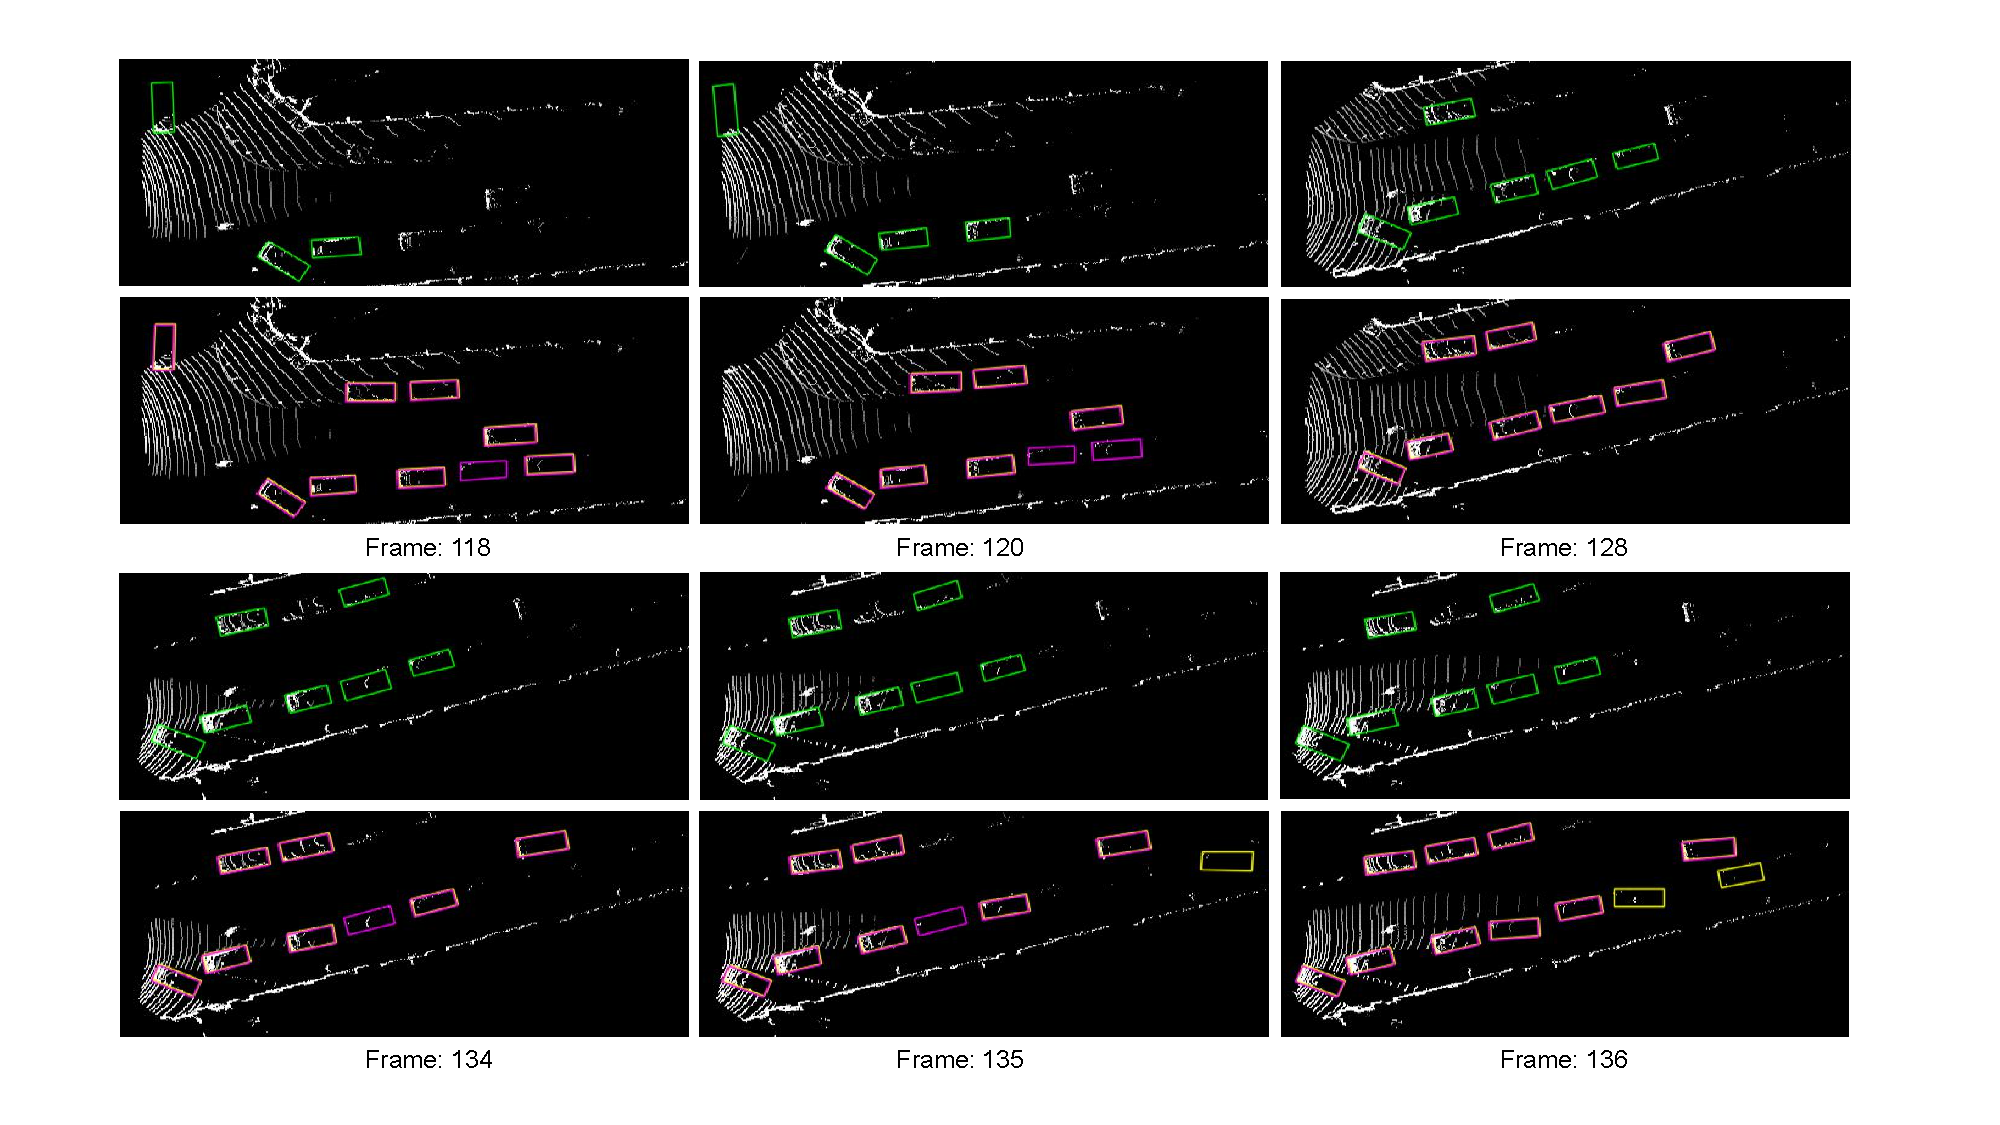
\includegraphics[trim={2cm, 1cm, 2cm, 1cm}, clip, width=\textwidth]{images/examples.pdf}
	\end{center}
	\caption{Visualization of labels and our predictions in sequences 0. Boxes in \textcolor{green}{\textbf{Green}} are official ground truth, boxes in \textcolor{yellow}{\textbf{Yellow}} are results predicted with temporal stride $\tau = 1$, and boxes in \textcolor{magenta}{\textbf{Magenta}} are results predicted with temporal stride $\tau = 3$. Best viewed in color.}
	\setlength{\belowcaptionskip}{-0.2cm}
	\label{fig:examples}
	\vspace{-0.4cm}
\end{figure*}

Secondly, We investigate the effect of multi-frame input. Specifically, we focus on the effect of different temporal strides $\tau$  on inference accuracy and speed. Towards this goal, we train six models with $\tau = \{1, 2, 3, 4, 5, 6\}$ respectively, and then link the predicted detections over time and generate detections in intermediate frames by box interpolation. Results are shown in \tablename \, \ref{table:result_detection}. DODT ($\tau = 2$) shows the best result in \textit{Easy} and \textit{Moderate} settings with IoU = 0.7, by 88.90\% and 76.64\% in $AP_{3D}$ respectively. While DODT ($\tau = 3$) shows the best performance in \textit{Hard} setting, with 75.84\% in $AP_{3D}$. Compared with the base model DODT ($\tau = 1$), the model performances with $\tau = 2, 3$ are boosted significantly in hard objects, by about 1\% in \textit{Moderate} setting and about 7\% in \textit{Hard} setting with IoU = 0.7.  This gain demonstrates that the detection of truncated and occluded targets can benefit greatly from a large temporal stride. Bottom two rows in \figurename \, \ref{fig:examples} shows how our interpolation algorithm improves model performance. Boxes in magenta are DODT predictions with $\tau = 3$ while yellow are with $\tau = 1$. The results shows that a larger $\tau$ can reduce noise and generate more true positive predictions. However,  \tablename \, \ref{table:result_detection} also shows that a too large $\tau$ leads to a significant decay of accuracy. As temporal stride increasing, there are more trajectories start or end within two keyframes, thus box interpolation would introduce more false positive predictions. 

We also compute the inference time in streaming level detection. The inference time for two keyframe inputs is 0.175s. As temporal stride $\tau$ increasing, the time cost for detection is unchanged, and interpolation time cost increases negligible, thus the inference time is almost the same, but FPS increases by multiple. We chose $\tau = 3$ for our following experiment, which is a good trade-off between inference speed and accuracy.

\begin{table}
	\resizebox{0.5\textwidth}{!}{
		\begin{tabular}{cccccccc}
			\toprule[1pt]
			Methods   & Modules & MOTA(\%)$\uparrow$ & MOTP(\%)$\uparrow$ & MT(\%)$\uparrow$ & ML(\%)$\downarrow$ & IDS$\downarrow$&  FRAG$\downarrow$ \\ \midrule
			DODT($\tau$ = 3)          & -      & 72.09    & 81.84    & 58.15  & 12.31  & 233    &  756  \\
			DODT($\tau$ = 3)          & T      & 73.26    & 82.38    & 58.61  & 12.00  & 340    &  699  \\
			DODT($\tau$ = 3)          & M      & 74.36    & \textbf{82.49}    & 56.66  & 13.08  & \textbf{27}   &  \textbf{310}  \\
			DODT($\tau$ = 3)          & T+M    & \textbf{76.68}    & 81.64    & \textbf{60.77}  & \textbf{11.69}  & 63  &  384  \\ 
			\bottomrule[1pt]
	\end{tabular}}
	\caption{Ablation study on KITTI Tracking test datasets.}
	\label{label:result_tracking}
\end{table}

\begin{table}
	\vspace{-0.3cm}
	\resizebox{0.5\textwidth}{!}{
		\begin{tabular}{cccccccc}
			\toprule[1pt]
			Method    & MOTA(\%)$\uparrow$ & MOTP(\%)$\uparrow$ & MT(\%)$\uparrow$ & ML(\%)$\downarrow$ & IDS$\downarrow$&  FRAG$\downarrow$ &FPS$\uparrow$ \\ \midrule
			Complexer-YOLO\cite{Simon_2019_CVPR_Workshops}    & 75.70    & 78.46    & 58.00  & 5.08  & 1186 & 2096 & 100.0 \\ %Complexer-YOLO
			DSM\cite{frossard2018end}                         & 76.15    & 83.42    & 60.00  & 8.31  & 296  & 868  & 10.0 (GPU)  \\ %DSM
			3D-CNN/PMBM\cite{scheidegger2018mono}             & 80.39    & 81.26	& 62.77  & 6.15  & 121  & 613  & 71.4 \\  %3D-CNN/PMBM
			3DT\cite{Hu3DT19} 	                              & \textbf{84.52}    & \textbf{85.64}	& \textbf{73.38}  & \textbf{2.77}  & 377  & 847  & 33.3 \\ %3DT
			DODT(ours)                                        & 76.68    & 81.65    & 60.77  & 11.69 & \textbf{63}   & \textbf{384}  & 100.0 \\ 
			\bottomrule[1pt]
	\end{tabular}}
	%\setlength{\abovecaptionskip}{1pt}
	\caption{Comparison of publicly available methods in the KITTI Tracking Benchmark. The time for object detection is not included in the specified runtime.}
	\label{label:result_kitti}
	%\vspace{-0.3cm}
\end{table}

\textbf{Multi-object tracking.} For multi-object tracking, We first investigate the contribution of different modules to tracking accuracy in KITTI tracking test datasets, results are shown in \tablename \, \ref{label:result_tracking}. The results shows that both modules can improve tracking performance. With these modules, our model outperforms base model by a large margin in nearly all tracking metrics (e.g. MOTA by 4.59\%, MT by 2.62\%, ML by -0.62\%, IDS by -170 and FRAG by -372), as \textit{Temporal Module} makes the data association more precise, and box interpolation can help to complete the track notably.  

We also compare our approach to publicly available methods of multiple object tracking in 3D in KITTI Tracking Benchmark, results are shown in \tablename \, \ref{label:result_kitti}. We can see that our approach is competitive with the state-of-the-art. For multiple object tracking accuracy, our method outperforms Complexer-YOLO \cite{Simon_2019_CVPR_Workshops} and DSM \cite{frossard2018end}, but behind 3D-CNN/PMBM \cite{scheidegger2018mono} and 3DT \cite{Hu3DT19}; For trajectory ID-switches and fragmentations, our method outperforms all other methods. Note that 3D-CNN/PMBM utilizes PMBM filter for data association while ours is a simple IoU based method, and 3DT trained their system on a new datasets collected on a realistic 3D virtual environments. Moreover, labels of test datasets maybe incomplete just like the case in training datasets, thus the tracking performance of our approach maybe better than current ones. Also, our approach shows a competitive results in runtime.

%%%%%%%%%%%%%%%%%%%%%%%%%%%%%%%%%%%%%%%%%%%%%%%%%%%%%%%%%%%%%%%%%%%%%%%%%%%%%%%%
\section{CONCLUSIONS}
\label{sec:conclusions} We propose DODT, a unified framework for simultaneous 3D object detection and tracking based on streaming data. The network is a dual-way structure and can  process two keyframes at the same time. Embedded with a \textit{Temporal Module} to encode the diversity of adjacent keyframes and a motion based interpolation algorithm to generate predictions in non-key frames, our network can overcome the challenge of target occlusion and loss in one frame, and perform object detection and tracking in a very efficient way. 

%Our approach achieves accuracy competitive with the state-of-the-art methods in KITTI Tracking Benchmark. 
%%%%%%%%%%%%%%%%%%%%%%%%%%%%%%%%%%%%%%%%%%%%%%%%%%%%%%%%%%%%%%%%%%%%%%%%%%%%%%%%

\bibliographystyle{IEEEtran}
\bibliography{IEEEabrv,egbib}
\end{document}
